\chapter[Thermal Model Development and Analysis Cases]
{Thermal Model Development in \\ ESATAN-TMS and Transient Analysis \\ Cases}
\label{ch:thermal_model}

The thermal model developed in \acrshort{esatan-tms} generates the results 
analysed throughout this work. It does not reproduce a particular flight 
design in full detail. Instead, it represents the main heat-transfer 
interactions with sufficient geometrical and physical detail to generate 
transient results and compare different cases. The same geometry, node 
hierarchy and thermal network are retained in every simulation, while the 
environmental and operating conditions are modified between cases.

The model contains the main body, two solar-panel wings, a camera, several 
internal electronic units, a battery, a radiator and \acrfull{mli}. Conductive 
and radiative couplings connect these elements, allowing temperatures and heat 
flows to be calculated throughout each simulation. The model follows the 
lumped-parameter formulation presented in 
\autoref{ch:theoretical_background} and implemented in 
\acrshort{esatan-tms} \cite{thermal_eng_man,esatan_user_man}.


\section{Model Development and Geometrical Configuration}
\label{sec:model_geometry}

The geometrical model is refined to represent the arrangement of the internal 
plates and equipment and the main conductive connections between them. This 
organisation also maintains a direct link between the physical elements and 
the node hierarchy used by the post-processing application.

The final internal configuration is shown from the $+Y$ and $-Y$ sides in 
Figure~\ref{fig:final_internal_model}. Both views show the 
distribution of the equipment across the structural plates and the different 
levels of the main body. The dissipative components represented in the model 
are the camera electronics, the battery, the \acrfull{obc}, the communications 
unit and the \acrfull{adcs}. Each unit is represented separately, allowing an 
individual internal heat load to be assigned and the corresponding temperature 
and heat exchanges to be analysed independently

The final external configuration is shown in
Figure~\ref{fig:final_external_model}. The main body presents a rectangular geometry 
and is divided into several surface nodes. Two solar-panel wings extend from 
opposite sides and are discretised independently. The camera assembly extends 
from the main body. Heat is rejected to space through the radiator, while the 
\acrshort{mli}-covered surfaces limit heat exchange with the external 
environment.

\begin{figure}[!htbp]
    \centering
    \phantomcaption

    \begin{subfigure}[c]{0.82\textwidth}
        \centering
        
\includegraphics[
            width=\linewidth,
            trim=0 45 0 45,
            clip
        ]{Image_02.png}
        \caption{Internal configuration viewed from the $+Y$ side.}
        \label{fig:internal_model_positive_y}
    \end{subfigure}
\end{figure}

\begin{figure}[!htbp]
    \ContinuedFloat
    \centering

    \begin{subfigure}[c]{0.72\textwidth}
        \centering
        
\includegraphics[
            width=\linewidth,
            trim=0 55 0 55,
            clip
        ]{Comp_disipativos.png}
        \caption{Internal configuration viewed from the $-Y$ side.}
        \label{fig:internal_model_negative_y}
    \end{subfigure}

    \caption{Internal configuration of the spacecraft thermal model viewed
    from opposite sides. The colours correspond to the geometry layer and do
    not represent temperatures.}
    \label{fig:final_internal_model}
\end{figure}

\begin{figure}[!htbp]
    \centering
    
\includegraphics[
        width=0.92\textwidth,
        trim=0 55 0 55,
        clip
    ]{Satelite.png}

    \caption{Final external configuration of the spacecraft thermal model in
    \acrshort{esatan-tms}. The colours correspond to the geometry layer and do
    not represent temperatures.}
    \label{fig:final_external_model}
\end{figure}

\FloatBarrier

\section{Thermal Model Hierarchy}
\label{sec:model_hierarchy}

The numerical nodes are grouped according to the physical elements they 
represent. This hierarchy consists of four levels:

\begin{itemize}
    \item \textbf{Level 0:} includes the complete \texttt{SAT\_AFM} model and 
    the \texttt{SPACE} boundary.

    \item \textbf{Level 1:} separates the main structure from the solar-panel 
    assembly.

    \item \textbf{Level 2:} divides the structure into the body, camera, 
    avionics and \acrshort{mli} groups.

    \item \textbf{Level 3:} contains the individual panels, structural plates, 
    camera elements and equipment units.
\end{itemize}

Each group is identified by a node range and a short label, giving a 
consistent naming system throughout the model. The \textit{Power} field 
indicates the equipment groups which have an internal heat load applied. 
The complete classification is given in 
\autoref{tab:subsystem-classification}.

% Uses packages already loaded in Tex_Files/packages.tex.

\begin{table}[H]
    \centering
    \caption{Thermal-model hierarchy and node identifiers.}
    \label{tab:subsystem-classification}

    \scriptsize
    \setlength{\tabcolsep}{2.5pt}
    \renewcommand{\arraystretch}{1.06}

    \begin{tabularx}{\textwidth}{
        |>{\raggedright\arraybackslash}X
        |c
        |>{\raggedright\arraybackslash}X
        |l
        |>{\raggedright\arraybackslash}X
        |c|
    }
        \hline
        \textbf{Group} &
        \textbf{Level} &
        \textbf{Parent} &
        \textbf{ID} &
        \textbf{Label} &
        \textbf{Power} \\
        \hline

        Space
        & 0 & None
        & \#99999
        & SPACE
        & False \\
        \hline

        SAT\_AFM
        & 0 & None
        & \#10000--75250
        & SAT\_AFM
        & False \\
        \hline

        STRUCTURE
        & 1 & SAT\_AFM
        & \#10000--51150
        & STR
        & False \\
        \hline

        SOLAR\_PANELS
        & 1 & SAT\_AFM
        & \#70000--75250
        & SP
        & False \\
        \hline

        BODY
        & 2 & STRUCTURE
        & \#10000--13650
        & STR\_BOD
        & False \\
        \hline

        CAMERA
        & 2 & STRUCTURE
        & \#40000--43750
        & STR\_CAM
        & False \\
        \hline

        AVIONICS
        & 2 & STRUCTURE
        & \#30000--35550
        & STR\_AV
        & False \\
        \hline

        MLI
        & 2 & STRUCTURE
        & \#50000--51150
        & STR\_MLI
        & False \\
        \hline

        SOLAR\_PANEL\_1
        & 3 & SOLAR\_PANELS
        & \#70000--72550
        & SP\_1
        & False \\
        \hline

        SOLAR\_PANEL\_2
        & 3 & SOLAR\_PANELS
        & \#73000--75250
        & SP\_2
        & False \\
        \hline

        BODY\_PANEL
        & 3 & BODY
        & \#10000--11150
        & STR\_BOD\_P
        & False \\
        \hline

        BODY\_PLATE\_INF
        & 3 & BODY
        & \#12000--12550
        & STR\_BOD\_PLI
        & False \\
        \hline

        BODY\_PLATE\_MED
        & 3 & BODY
        & \#12600--13050
        & STR\_BOD\_PLM
        & False \\
        \hline

        BODY\_PLATE\_SUP
        & 3 & BODY
        & \#13100--13650
        & STR\_BOD\_PLS
        & False \\
        \hline

        CAMERA\_BASE
        & 3 & CAMERA
        & \#40000--40450
        & STR\_CAM\_BASE
        & False \\
        \hline

        CAMERA\_ELEC
        & 3 & CAMERA
        & \#40500--41050
        & STR\_CAM\_ELEC
        & True \\
        \hline

        CAMERA\_LENS
        & 3 & CAMERA
        & \#41500--42150
        & STR\_CAM\_LENS
        & False \\
        \hline

        CAMERA\_CYL
        & 3 & CAMERA
        & \#42500--43550
        & STR\_CAM\_CYL
        & False \\
        \hline

        BATTERY
        & 3 & AVIONICS
        & \#30000--30550
        & STR\_AV\_BAT
        & True \\
        \hline

        OBC\_BOX
        & 3 & AVIONICS
        & \#31000--31550
        & STR\_AV\_OBC
        & True \\
        \hline

        COMMS\_BOX
        & 3 & AVIONICS
        & \#32000--32550
        & STR\_AV\_COM
        & True \\
        \hline

        ADCS\_UNIT
        & 3 & AVIONICS
        & \#33000--33550
        & STR\_AV\_ADCS
        & True \\
        \hline

        RADIATOR
        & 3 & AVIONICS
        & \#34000--35550
        & STR\_AV\_RAD
        & False \\
        \hline

        MLI\_PANELS
        & 3 & MLI
        & \#50000--51150
        & STR\_MLI\_P
        & False \\
        \hline
    \end{tabularx}
\end{table}

\begin{figure}[H]
    \centering
    \phantomcaption

    \begin{subfigure}[c]{0.78\textwidth}
        \centering
        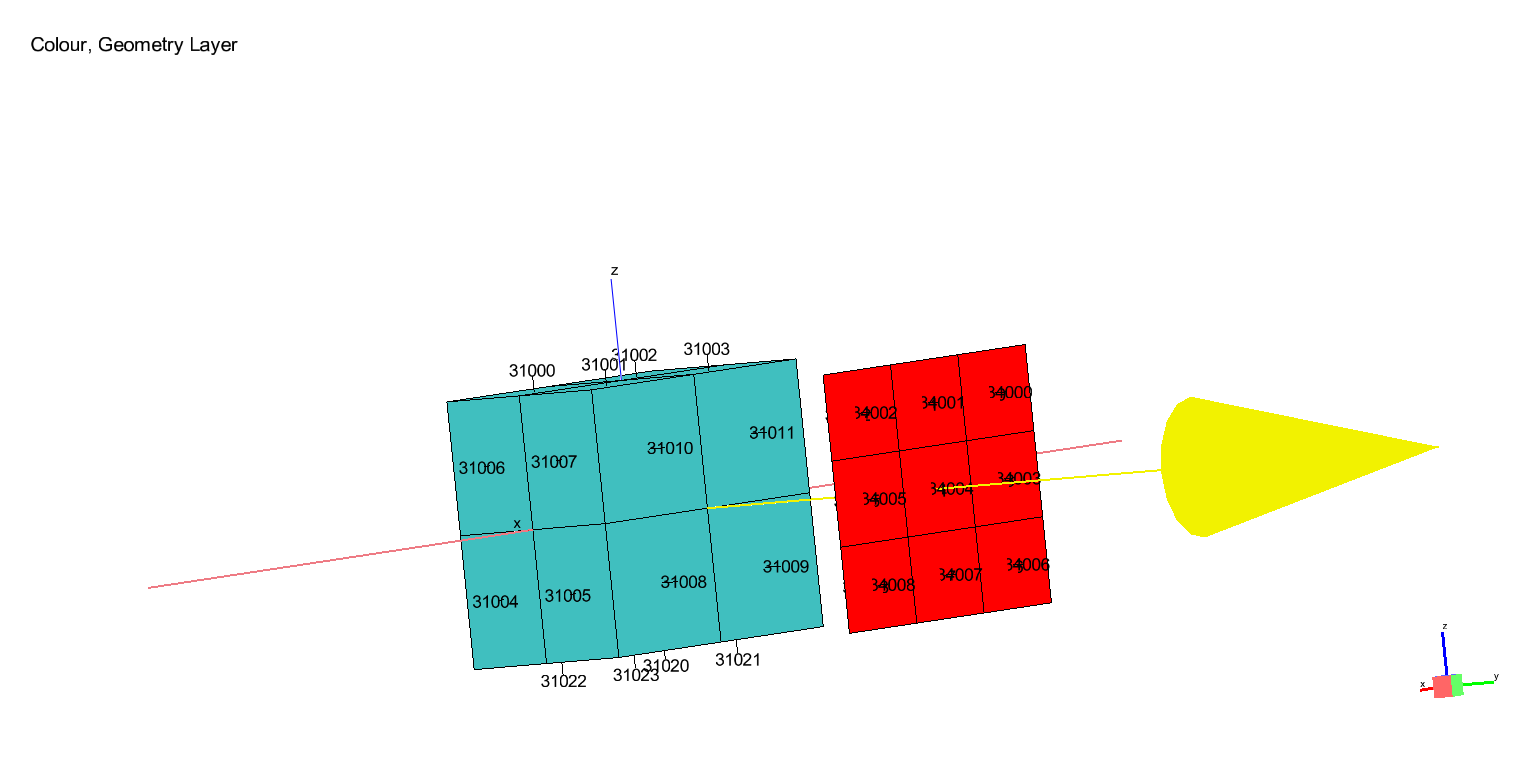
\includegraphics[width=\linewidth]
        {Figures/05/OBC_Rad_nodes.png}
        \caption{First view of the OBC and radiator nodal numbering.}
        \label{fig:obc_radiator_nodes_a}
    \end{subfigure}
\end{figure}

\begin{figure}[H]
    \ContinuedFloat
    \centering

    \begin{subfigure}[c]{0.78\textwidth}
        \centering
        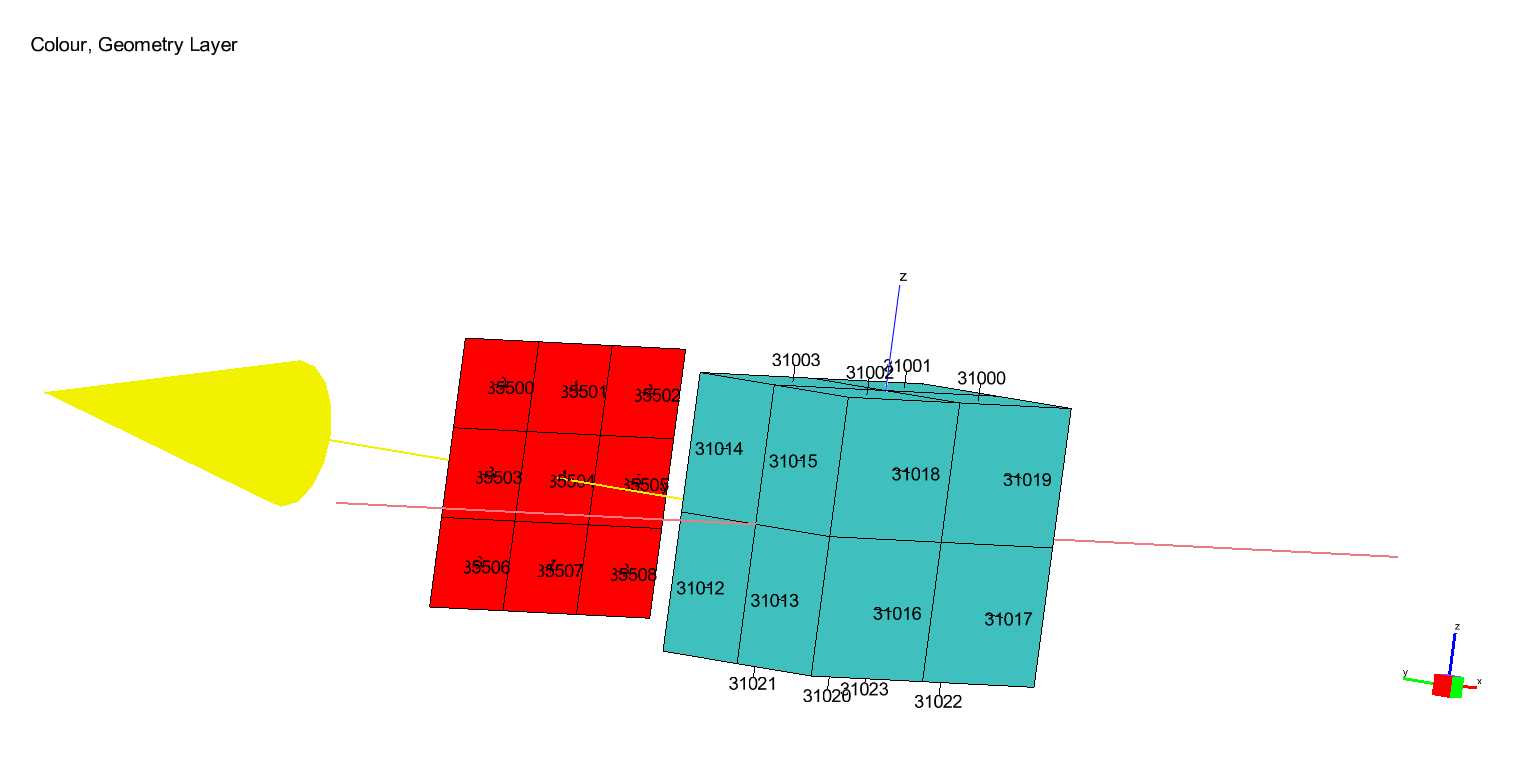
\includegraphics[width=\linewidth]
        {Figures/05/OBC_Rad_nodes2.png}
        \caption{Opposite view of the OBC and radiator nodal numbering.}
        \label{fig:obc_radiator_nodes_b}
    \end{subfigure}

    \caption{Example of nodal numbering for the OBC and adjacent radiator
    surfaces, shown from opposite sides. The figure illustrates the node
    ranges listed in Table~\ref{tab:subsystem-classification}.}
    \label{fig:obc_radiator_nodes}
\end{figure}

\section{Material and Surface Properties}
\label{sec:model_properties}

The temperature response of each geometrical element depends on the 
assigned bulk material and the thermo-optical properties of the surfaces. 
Thermal conductivity, density and specific heat capacity determine 
heat conduction and energy storage, while the surface properties govern the 
interaction with solar and infrared radiation. The same definitions are used 
in all analysis cases. Consequently, changes in the calculated results are 
associated with the environmental and operating inputs rather than with 
modifications to the model.


\subsection{Bulk Properties}
\label{subsec:bulk_properties}

The geometrical elements use four material definitions. Aluminium 6061 is 
assigned to the main structural panels, internal plates and equipment 
housings. Gallium arsenide represents the solar-cell elements, while a 
separate optical material is used for the camera lens. The 
\acrshort{mli} foil has an independent definition whose conductivity is set 
to zero. This prevents the geometrical shell from introducing a 
solid-conduction connection, while the intended couplings are defined 
explicitly in the thermal network.

The conductivity, specific heat capacity and density assigned to each material 
are listed in \autoref{tab:material-properties}. 
Figure~\ref{fig:conductivity_distribution} shows only the conductivity 
distribution, using two opposite views to cover the complete geometry. This 
allows the assignments to the structure, solar cells, camera and 
\acrshort{mli} surfaces to be checked.

% Uses packages already loaded in Tex_Files/packages.tex.

\begin{table}[H]
    \centering
    \caption{Material properties used in the thermal model.}
    \label{tab:material-properties}
    
    \small
    \setlength{\tabcolsep}{6pt}
    \renewcommand{\arraystretch}{1.12}
    \resizebox{0.7\textwidth}{!}{%
        \begin{tabular}{|l|c|c|c|}
            \hline
            \textbf{Name} &
            \(\boldsymbol{k}\,[\mathrm{W\,m^{-1}\,K^{-1}}]\) &
            \(\boldsymbol{c_p}\,[\mathrm{J\,kg^{-1}\,K^{-1}}]\) &
            \(\boldsymbol{\rho}\,[\mathrm{kg\,m^{-3}}]\) \\
            \hline

            Al\_6061 & 160 & 900 & 2700 \\
            \hline

            GaAs & 55 & 1000 & 5300 \\
            \hline

            Glass & 59 & 310 & 5330 \\
            \hline

            MLI\_foil & 0 & 900 & 300 \\
            \hline
        \end{tabular}
    }
\end{table}

\par\addvspace{32mm}

\begin{figure}[H]
    \centering
    \phantomcaption

        \begin{subfigure}[c]{0.8\textwidth}
        \centering
        
\includegraphics[
            width=\linewidth,
            trim=0 8 0 120,
            clip
        ]{thermal_conductivity2.png}
        \caption{View from the side $+Y$.}
        \label{fig:conductivity_distribution_opposite}
    \end{subfigure}
\end{figure}

\begin{figure}[H]
    \ContinuedFloat
    \centering

    \begin{subfigure}[c]{0.7\textwidth}
        \centering
        
\includegraphics[
            width=\linewidth,
            trim=0 8 0 120,
            clip
        ]{thermal_conductivity.png}
        \caption{View from side $-Y$.}
        \label{fig:conductivity_distribution_view_a}
    \end{subfigure}

    \caption{Thermal conductivity distribution over the final spacecraft
    model, viewed from opposite sides.}
    \label{fig:conductivity_distribution}
\end{figure}

\FloatBarrier


\subsection{Thermo-optical Properties}
\label{subsec:thermo_optical_properties}

The surface definitions are assigned according to the function of each 
element. Anodised aluminium is used on selected structural surfaces, while 
black paint is applied to the internal equipment. An \acrfull{osr} defines the 
radiator surface, and the solar cells use a separate coating definition. The 
external \acrshort{mli} is represented by Kapton coated with 
\acrfull{ito}, while independent properties are assigned to the internal 
\acrshort{mli} and the infrared lens.

The solar and infrared bands are defined separately. For each surface, the 
model specifies absorptivity or emissivity, transmissivity and the specular 
and diffuse components of reflectivity. Within each band, these coefficients 
are defined so that the corresponding energy fractions sum to unity.

The adopted solar absorptivity and infrared emissivity values are consistent 
with representative measurements compiled for black coatings, anodised 
aluminium, solar cells, optical solar reflectors and Kapton films 
\cite{kauder2005coatings}. These data are used as 
reference values, since a single nominal definition 
is assigned to each surface in the model. The complete set of properties is summarised in
\autoref{tab:thermo-optical-properties}.
% Source locations: printed pages 40, 43, 46 and 48;
% PDF pages 46, 49, 52 and 54.

% Uses packages already loaded in Tex_Files/packages.tex.

\begin{table}[H]
    \centering
    \caption{Thermo-optical coating properties used in the thermal model.}
    \label{tab:thermo-optical-properties}

    \setlength{\tabcolsep}{3pt}
    \renewcommand{\arraystretch}{1.15}
    
    \resizebox{0.6\textwidth}{!}{%
        \begin{tabular}{|l|*{8}{c|}}
            \hline
            \multirow{2}{*}{\textbf{Name}} &
            \multicolumn{4}{c|}{\textbf{Infrared}} &
            \multicolumn{4}{c|}{\textbf{Solar}} \\
            \cline{2-9}

            &
            \(\boldsymbol{\varepsilon}\) &
            \(\boldsymbol{\tau}\) &
            \(\boldsymbol{\rho_{\mathrm{spec}}}\) &
            \(\boldsymbol{\rho_{\mathrm{diff}}}\) &
            \(\boldsymbol{\alpha}\) &
            \(\boldsymbol{\tau}\) &
            \(\boldsymbol{\rho_{\mathrm{spec}}}\) &
            \(\boldsymbol{\rho_{\mathrm{diff}}}\) \\
            \hline

            Al anodized
            & 0.6 & 0 & 0 & 0.4
            & 0.2 & 0 & 0 & 0.8 \\
            \hline

            Black paint
            & 0.9 & 0 & 0 & 0.1
            & 0.9 & 0 & 0 & 0.1 \\
            \hline

            OSR
            & 0.8 & 0 & 0.2 & 0
            & 0.08 & 0 & 0.92 & 0 \\
            \hline

            Solar cells
            & 0.75 & 0 & 0 & 0.25
            & 0.75 & 0 & 0 & 0.25 \\
            \hline

            IR lens
            & 0.1 & 0.9 & 0 & 0
            & 0.5 & 0 & 0 & 0.5 \\
            \hline

            Kapton ITO
            & 0.8 & 0 & 0 & 0.2
            & 0.5 & 0 & 0 & 0.5 \\
            \hline

            MLI\_int
            & 0.2 & 0 & 0 & 0.8
            & 0.2 & 0 & 0 & 0.8 \\
            \hline
        \end{tabular}
    }   
\end{table}

The solar absorptivity and reflectivity distributions are presented in
Figures~\ref{fig:solar_absorptivity_distribution}
and~\ref{fig:solar_reflectivity_distribution}. Higher absorptivity is assigned 
to the solar cells and black-painted surfaces, whereas the radiator 
\acrshort{osr} has the lowest value. The reflectivity maps show the 
corresponding distribution of reflected solar energy. Two opposite views are 
included for each property so that the assignments can be checked over the 
complete geometry.

\begin{figure}[!htbp]
    \centering
    \phantomcaption

    \begin{subfigure}[c]{1.0\textwidth}
        \centering
        
\includegraphics[width=\linewidth]
        {solar_absorptivity.png}
        \caption{View from one side.}
        \label{fig:solar_absorptivity_distribution_view_a}
    \end{subfigure}
\end{figure}

\begin{figure}[!htbp]
    \ContinuedFloat
    \centering

    \begin{subfigure}[c]{1.0\textwidth}
        \centering
        
\includegraphics[width=\linewidth]
        {solar_absorptivity2.png}
        \caption{View from the opposite side.}
        \label{fig:solar_absorptivity_distribution_opposite}
    \end{subfigure}

    \caption{Solar absorptivity distribution over the final spacecraft
    model, viewed from opposite sides.}
    \label{fig:solar_absorptivity_distribution}
\end{figure}

\begin{figure}[!htbp]
    \centering
    \phantomcaption

    \begin{subfigure}[c]{1.0\textwidth}
        \centering
        
\includegraphics[width=\linewidth]
        {solar_reflectivity.png}
        \caption{View from one side.}
        \label{fig:solar_reflectivity_distribution_view_a}
    \end{subfigure}
\end{figure}

\begin{figure}[!htbp]
    \ContinuedFloat
    \centering

    \begin{subfigure}[c]{1.0\textwidth}
        \centering
        
\includegraphics[width=\linewidth]
        {solar_reflectivity2.png}
        \caption{View from the opposite side.}
        \label{fig:solar_reflectivity_distribution_opposite}
    \end{subfigure}

    \caption{Solar reflectivity distribution over the final spacecraft
    model, viewed from opposite sides.}
    \label{fig:solar_reflectivity_distribution}
\end{figure}

\FloatBarrier

The infrared emissivity and reflectivity distributions are shown in
Figures~\ref{fig:infrared_emissivity_distribution}
and~\ref{fig:infrared_reflectivity_distribution}. High emissivity is assigned 
to the black-painted surfaces and the radiator, promoting radiative heat 
exchange. Lower values are used for the internal \acrshort{mli} and the camera 
lens, which also includes infrared transmissivity. These assignments determine 
the radiative exchange between internal elements and the rejection of heat 
from the external surfaces.

\begin{figure}[!htbp]
    \centering
    \phantomcaption

    \begin{subfigure}[c]{1.0\textwidth}
        \centering
        
\includegraphics[width=\linewidth]
        {infrarred_emmisivity.png}
        \caption{View from one side.}
        \label{fig:infrared_emissivity_distribution_view_a}
    \end{subfigure}
\end{figure}

\begin{figure}[!htbp]
    \ContinuedFloat
    \centering

    \begin{subfigure}[c]{1.0\textwidth}
        \centering
        
\includegraphics[width=\linewidth]
        {infrarred_emmisivity2.png}
        \caption{View from the opposite side.}
        \label{fig:infrared_emissivity_distribution_opposite}
    \end{subfigure}

    \caption{Infrared emissivity distribution over the final spacecraft
    model, viewed from opposite sides.}
    \label{fig:infrared_emissivity_distribution}
\end{figure}

\begin{figure}[!htbp]
    \centering
    \phantomcaption

    \begin{subfigure}[c]{1.0\textwidth}
        \centering
        
\includegraphics[width=\linewidth]
        {infrarred_reflectivity.png}
        \caption{View from one side.}
        \label{fig:infrared_reflectivity_distribution_view_a}
    \end{subfigure}
\end{figure}

\begin{figure}[!htbp]
    \ContinuedFloat
    \centering

    \begin{subfigure}[c]{1.0\textwidth}
        \centering
        
\includegraphics[width=\linewidth]
        {infrarred_reflectivity2.png}
        \caption{View from the opposite side.}
        \label{fig:infrared_reflectivity_distribution_opposite}
    \end{subfigure}

    \caption{Infrared reflectivity distribution over the final spacecraft
    model, viewed from opposite sides.}
    \label{fig:infrared_reflectivity_distribution}
\end{figure}

\FloatBarrier


\section{Nodal Discretisation and Thermal Network Definition}
\label{sec:thermal_network_definition}

The geometrical model is divided into nodes according to the spatial 
resolution required for the analysis. Large external elements, including the 
body panels and solar-panel wings, are represented by several nodes to capture 
local temperature differences and variations in the absorbed environmental loads. 
Internal plates and equipment units are also discretised separately to 
reproduce the main heat-transfer paths through the structure.

Each capacitive node is assigned a material, mass and specific heat capacity.
Following this nodal division, the conductive network represents 
heat transfer through the structure and between the internal equipment 
and supporting plates. Most conductive 
paths correspond to physical contacts included in the geometry. When a physical 
connection is not represented geometrically, an additional conductor is defined. 
This is the case for the thermal link between the \acrshort{obc} and the radiator, 
which is included without adding unnecessary geometrical detail.

The radiative network represents exchange between the relevant surfaces and with the 
deep-space boundary.

Internal heat loads are applied to the nodes representing the dissipative equipment. 
The values assigned in each transient case are summarised in 
Table~\ref{tab:internal_heat_loads}. The battery load is defined separately
for eclipse and non-eclipse intervals.

\begin{table}[htbp]
    \centering
    \caption{Internal heat loads applied in the selected transient cases.}
    \label{tab:internal_heat_loads}

    \small
    \setlength{\tabcolsep}{5pt}
    \renewcommand{\arraystretch}{1.15}

    \begin{tabularx}{\textwidth}{
        |>{\raggedright\arraybackslash}X
        |*{3}{>{\centering\arraybackslash}p{0.19\textwidth}|}
    }
        \hline
        \multirow{2}{*}{\textbf{Component}} &
        \multicolumn{3}{c|}{\textbf{Applied power (W)}} \\
        \cline{2-4}

        &
        \textbf{Nominal} &
        \textbf{Hot} &
        \textbf{Cold} \\
        \hline

        Camera electronics
        & 2.00
        & 3.50
        & 0.00 \\
        \hline

        Battery, outside eclipse
        & 1.50
        & 2.06
        & 0.375 \\
        \hline

        Battery, during eclipse
        & 10.00
        & 13.75
        & 2.50 \\
        \hline

        \acrshort{obc}
        & 4.00
        & 5.00
        & 2.00 \\
        \hline

        Communications unit
        & 3.00
        & 4.50
        & 0.50 \\
        \hline

        \acrshort{adcs}
        & 2.00
        & 3.50
        & 0.50 \\
        \hline
    \end{tabularx}
\end{table}

The node definitions and conductive and radiative couplings remain unchanged in all 
transient cases. Only the environmental conditions and internal heat loads 
are modified as requires for each case. Consequently, each node and thermal coupling 
represents the same physical element in every exported result file, allowing direct 
comparison between cases.


\section{Orbital Environment and Radiative Cases}
\label{sec:radiative_cases}

The orbital environment defines the external radiative conditions applied to
the model. Direct solar radiation, planetary albedo and planetary infrared
emission are included as external heat inputs \cite{ecss_st_10_04c}. Energy
emitted by the external surfaces towards deep space is also considered. These
exchanges are represented through the orbital and radiative models of
\acrshort{esatan-tms} and provide the boundary conditions used in the
transient simulations \cite{thermal_eng_man}.

Three radiative cases are selected: \texttt{rad\_nominal},
\texttt{rad\_hot\_operational} and
\texttt{rad\_cold\_operational}. The same geometry and surface properties are
retained in all three cases, while the environmental parameters and eclipse
duration differ between them. For the radiative calculation, each orbital
revolution is divided into 24 positions separated by \(15^{\circ}\). This
common angular sampling allows the incident loads to be evaluated consistently
throughout the orbit and included in the transient solution.

Figure~\ref{fig:nominal_orbit_positions} shows the orbital configuration of
the nominal case. The spacecraft positions illustrate the discretisation used
for the radiative calculation. The green segment represents the portion
outside eclipse, whereas the red segment identifies the eclipse interval.

\begin{figure}[H]
    \centering
    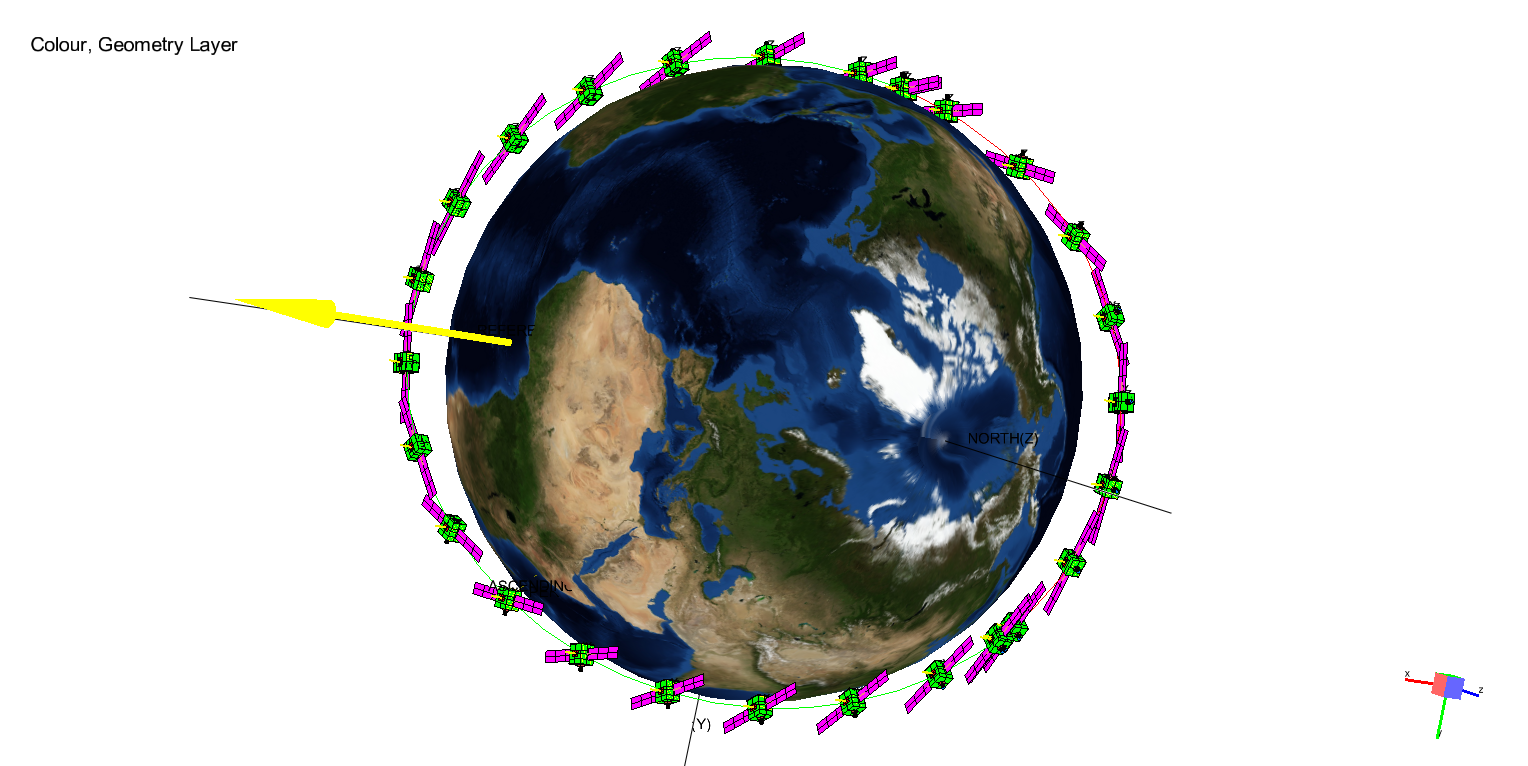
\includegraphics[width=1.0\textwidth]
    {Figures/05/nominal_orbit_positions.png}
    \caption{Nominal orbital configuration and the 24 positions used for the
    radiative calculation. The green segment represents the portion outside
    eclipse, while the red segment indicates the eclipse interval.}
    \label{fig:nominal_orbit_positions}
\end{figure}

The \texttt{rad\_nominal} case provides the reference environment.
\texttt{rad\_hot\_operational} combines a higher external heat input with a
shorter eclipse, whereas \texttt{rad\_cold\_operational} combines a lower
input with a longer eclipse.

These environments provide clearly differentiated conditions for comparing
the hot and cold responses with the nominal case without modifying the
physical model. They are selected for the analyses performed in this work and
do not cover every condition expected during a flight mission.

\section{Transient Analysis Cases}
\label{sec:transient_cases}

\subsection{Definition of Analysis Cases}
\label{subsec:analysis_case_definition}

Three transient simulations are selected for the final analysis: nominal, hot
and cold. The nominal case provides the reference response, while the hot and
cold cases represent higher and lower external heat inputs, respectively.
Different equipment loads are also assigned according to the operating
conditions defined for each simulation. Their purpose is summarised in
Table~\ref{tab:transient_cases}.

\begin{table}[htbp]
    \centering
    \caption{Transient cases selected from the common thermal model.}
    \label{tab:transient_cases}

    \small
    \setlength{\tabcolsep}{6pt}
    \renewcommand{\arraystretch}{1.15}

    \begin{tabularx}{\textwidth}{
        |>{\raggedright\arraybackslash}p{0.17\textwidth}
        |>{\raggedright\arraybackslash}p{0.27\textwidth}
        |>{\raggedright\arraybackslash}X|
    }
        \hline
        \textbf{Case} &
        \textbf{Radiative case} &
        \textbf{Purpose} \\
        \hline

        Nominal &
        \texttt{rad\_nominal} &
        Reference response used for comparison with the hot and cold cases. \\
        \hline

        Hot &
        \texttt{rad\_hot\_operational} &
        Response under higher external heat input and a shorter eclipse. \\
        \hline

        Cold &
        \texttt{rad\_cold\_operational} &
        Response under lower external heat input and a longer eclipse. \\
        \hline
    \end{tabularx}
\end{table}

The same geometry, materials, surface properties, node labels, hierarchy and
thermal couplings are retained in all three simulations. Only the radiative
environment and internal heat loads change between cases. Equivalent nodes and
variables therefore retain the same physical meaning, allowing the hot and
cold results to be compared directly with the nominal case.


\subsection{Solver Configuration and Temporal Sampling}
\label{subsec:solver_sampling}

The \textit{Solution Control} configuration applied to the three analysis
cases is shown in Figure~\ref{fig:solver_execution_block}.

\begin{figure}[htbp]
    \centering
    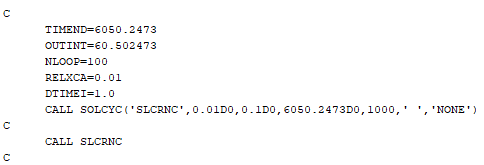
\includegraphics[width=0.9\textwidth]
    {Figures/05/solver_execution_block.png}
    \caption{\textit{Solution Control} execution block used to obtain cyclic
    convergence and calculate the final transient orbital period in
    \acrshort{esatan-tms}.}
    \label{fig:solver_execution_block}
\end{figure}

\begin{samepage}

The same numerical settings are used in all three simulations. The transient
solution is calculated using the Crank--Nicolson method. Before the final
results are exported, \texttt{SOLCYC} repeats the orbital period until the
maximum difference between the initial and final nodal temperatures is below
\(0.01\,^{\circ}\mathrm{C}\). A maximum of 1000 cycles is allowed. The
converged temperature field is then used as the initial condition for the
orbital period retained for analysis.

Each exported simulation covers \(6050.247\,\mathrm{s}\) and contains 101
output instants separated by approximately \(60.50\,\mathrm{s}\). This common
time basis records the main changes in the applied loads and allows values
from different cases to be compared at equivalent points of the orbit.

\end{samepage}


\section{Thermal Model Verification}
\label{sec:thermal_model_verification}

Verification is performed throughout model development using visual and
numerical checks. The material and surface-property maps are inspected to
identify missing or incorrectly assigned faces. The node hierarchy is 
compared with the physical arrangement to confirm that the external panels,
internal plates and equipment units belong to the correct model groups.

The conductive and radiative networks are reviewed to identify isolated nodes,
missing links and unintended heat-transfer paths. Nodal energy balances are
examined to detect inconsistent loads or exchanges. Finally, the exported
results are checked to confirm that every selected case satisfies the required
cyclic-convergence criterion.

These checks confirm the internal consistency of the model but do not validate it
against experimental data. No corresponding flight hardware or thermal-vacuum
test data are available for comparison. The conclusions are therefore limited
to the behaviour predicted by the model under the defined environmental and
operating conditions.


\section{Simulation Results Export in TMD Format}
\label{sec:tmd_export}

After each simulation is completed, the result set obtained for each case is exported from
\acrshort{esatan-tms} as a separate \texttt{.TMD} file. Each file stores the
time vector and the nodal quantities selected for post-processing, including
temperatures, applied loads, absorbed environmental loads, and conductive and
radiative heat flows. Node numbers and labels are preserved during export,
allowing each variable to be associated with the corresponding group in the
external hierarchy spreadsheet.

The structural and temporal dimensions shared by the three result files are
summarised in Table~\ref{tab:tmd_summary}. The nominal, hot and cold files
retain the same node and conductor structure and cover a common time
interval.

Together, the three files form the dataset used for the transient and
multi-case analyses. Their common structure allows equivalent variables to
be represented at the same orbital instants and compared directly with
respect to the nominal case.

\begin{table}[H]
    \centering
    \caption{Structural and temporal characteristics of the exported
        \texttt{.TMD} files.}
    \label{tab:tmd_summary}
    \small
    \setlength{\tabcolsep}{8pt}
    \renewcommand{\arraystretch}{1.15}

    \begin{tabularx}{0.76\textwidth}{|X|c|}
        \hline
        Total thermal nodes per file
        & 284 \\
        \hline

        Capacitive nodes
        & 282 \\
        \hline

        Boundary nodes
        & 1 \\
        \hline

        Inactive nodes
        & 1 \\
        \hline

        Linear conductors, \(G^{L}\)
        & 597 \\
        \hline

        Radiative conductors, \(G^{R}\)
        & 3292 \\
        \hline

        Time interval
        & \(6050.247\,\mathrm{s}\) \\
        \hline

        Output instants per file
        & 101 \\
        \hline

        Approximate output time step
        & \(60.502\,\mathrm{s}\) \\
        \hline
    \end{tabularx}
\end{table}

The 101 output instants correspond to the temporal sampling of the transient
solution and should not be confused with the 24 orbital positions used in the
radiative calculation. For each nodal variable, one file therefore contains
\(284 \times 101 = 28\,684\) values before the conductor results and remaining
nodal quantities are considered.

The absorbed solar loads calculated for the solar panels are also retained in
the exported data. These values are used as inputs for the
electrical-generation and battery calculations. This processing is
performed independently and does not modify the \acrshort{esatan-tms}
solution.

The three \texttt{.TMD} files and the hierarchy spreadsheet form the input
dataset used by the Python application to read, organise and compare the
results.